\documentclass[12pt,fleqn,answers]{exam}
\usepackage{amssymb}
\usepackage[intlimits]{amsmath}
\usepackage{epsfig}
\usepackage{upgreek}
\usepackage[super]{nth}
\usepackage[colorlinks=true,linkcolor=black,anchorcolor=black,citecolor=black,filecolor=black,menucolor=black,runcolor=black,urlcolor=black]{hyperref}
\usepackage[letterpaper, margin=0.75in]{geometry}
\addpoints
\boxedpoints
\pointsinmargin
\pointname{pts}
\usepackage{tikz}
\usepackage{tkz-euclide}
\usetikzlibrary{shapes.geometric}
\usetikzlibrary{calc}
\usepackage[final]{microtype}
\usepackage[american]{babel}
\usepackage[T1]{fontenc}
\usepackage[]{fourier}

\usepackage{isomath}
\usepackage{upgreek,amsmath}
\usepackage{graphicx}

\newcommand{\dotprod}{\, {\scriptzcriptztyle\stackrel{\bullet}{{}}}\,}

\newcommand{\reals}{\mathbf{R}}
\newcommand{\lub}{\mathrm{lub}} 
\newcommand{\glb}{\mathrm{glb}} 
\newcommand{\complex}{\mathbf{C}}
\newcommand{\dom}{\mbox{dom}}
\newcommand{\range}{\mbox{range}}
\newcommand{\cover}{{\mathcal C}}
\newcommand{\integers}{\mathbf{Z}}
\newcommand{\vi}{\, \mathbf{i}}
\newcommand{\vj}{\, \mathbf{j}}
\newcommand{\vk}{\, \mathbf{k}}
\newcommand{\bi}{\, \mathbf{i}}
\newcommand{\bj}{\, \mathbf{j}}
\newcommand{\bk}{\, \mathbf{k}}
\DeclareMathOperator{\Arg}{\mathrm{Arg}}
\DeclareMathOperator{\Ln}{\mathrm{Ln}}
\newcommand{\imag}{\, \mathrm{i}}
\newcommand{\erf}{\mathrm{erf}}
\newcommand{\e}{\mathrm{e}}

\usepackage{graphicx}
\usepackage{color}
%\shadedsolutions
%\definecolor{SolutionColor}{rgb}{1,0.72,0.46} %{0.8,0.9,1}
\newcommand\AM{\textsc{am}}
\newcommand\PM{\textsc{pm}}


     
\newcommand{\quiz}{25}
\newcommand{\term}{Fall}
\newcommand{\due}{Thursday 30 November at 13:20}
\newcommand{\class}{MATH 202, Fall \the\year}
\begin{document}
\large
\noindent\makebox[3.0truein][l]{\textbf{\class}}
\textbf{Name:} \hrulefill \\
\noindent \makebox[3.0truein][l]{\textbf{In class work  \quiz}}
\textbf{Row and Seat}:\hrulefill\\



\noindent  In class work  \textbf{\quiz}  has questions \textbf{1} 
through  \textbf{\numquestions} \/ with a total of 
\textbf{\numpoints\/} points. Turn in your work at the end of class 
\emph{on paper}. This assignment is due \emph{\due}.

\vspace{0.1in}

\noindent \emph{“As we express our gratitude, we must never forget that the highest 
appreciation is not to utter words, but to live by them.”} 
  \hfill {\sc John F. Kennedy}


\begin{questions} 
    
  



\question In polar coordinates, an equation of a curve 
$\mathcal{C}$ is $r = \sqrt{\frac{1}{4} - \sin(\theta)^2}$.

\begin{parts}

\part[2] Use Desmos to draw a graph of this polar equation. As best you
can, reproduce the graph here.

\begin{solution}[2.5in]
    The curve is a Lemniscate of Booth. It looks like the infinity 
    symbol. Its graph is shown below.

    \begin{center}
        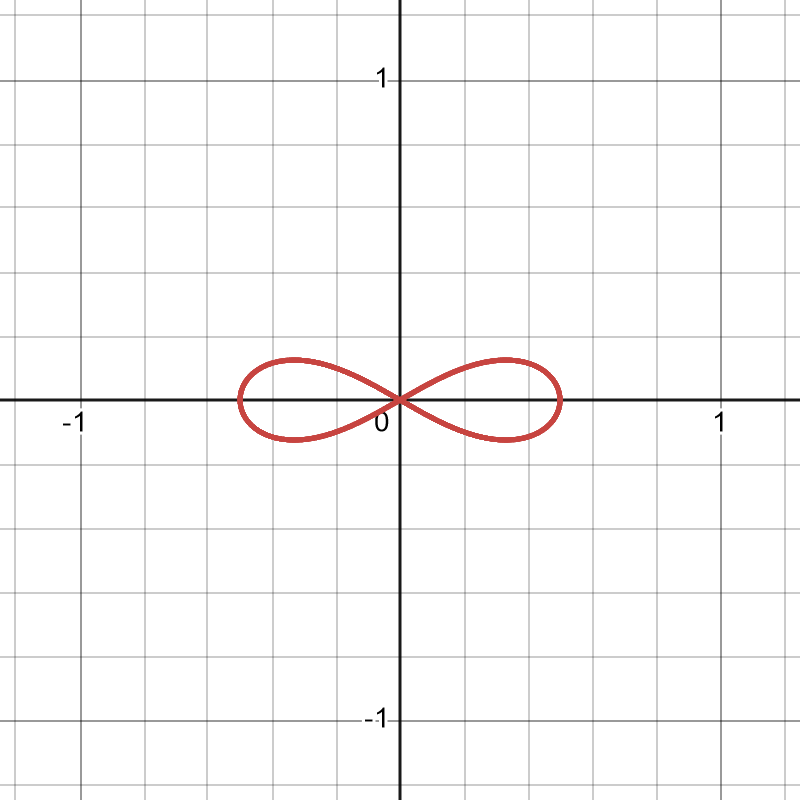
\includegraphics[scale=0.15]{desmos-graph(70).png}
    \end{center}

    Notice that the natural domain of $r = \sqrt{\frac{1}{4} - \sin(\theta)^2}$
    is $\theta \in [-\frac{\uppi}{6}, -\frac{\uppi}{6}] \cup 
    [\frac{5 \uppi}{6}, \frac{7\uppi}{6}]$; outside this 
    set, the value of $r$ is not real. Desmos recognizes this and skips
    over the territory where $r$ isn't real. 
  
\end{solution}

\part[2] Find all solutions to $0 = \sqrt{\frac{1}{4} - \sin(\theta)^2}$ 
with $\theta \in [0, 2 \uppi]$.
These solutions give all the points on the curve that intersect 
the origin.  To find \emph{all} solutions to this
equation, use the \emph{source of all knowledge} (\textbf{SOAK}), that is, 
the unit circle.

\begin{solution}%[2.5in] We need to solve
    \begin{align*}
        \left [0 = \sqrt{\frac{1}{4} - \sin(\theta)^2} \right ] &=
            \left [ 0=\frac{1}{4} - \sin(\theta)^2 \right ], && (\text{square root fact}) \\
            &=\left [0=\left(\frac{1}{2} - \sin(\theta)\right) \left(\frac{1}{2} +\sin(\theta) \right) \right], && (\text{factor}) \\
            &= \left [ -\frac{1}{2}=\sin(\theta) \lor
            -\frac{1}{2}=\sin(\theta)
            \right ], && (\text{factor and solve})\\
            &= \left[ \theta=\frac{11 \uppi}{6},
                 \theta=\frac{\uppi}{6},\theta=\frac{5\uppi}{6},
                 \theta=\frac{7 \uppi}{6} \right]. && (\text{SOAK})
    \end{align*}
\end{solution}

%\newpage

\part[2] For each intersection of $\mathcal{C}$ with the origin, find
the slope of the tangent line. Using Desmos, verify that 
you have found the correct tangent lines. \textbf{Note:} Desmos
refuses\footnote{I think Desmos should hire some UNK CS graduates 
to fix this.} to graph a polar curve of the form $\theta = f(r)$. 
And it particular, it will not graph the polar curve 
$\theta = \frac{\uppi}{4}$,  for example. To workaround this,
you'll need to find the cartesian equation of the tangent lines.

\begin{solution}
    For the polar curve $r = f(\theta)$ and assuming $f(\theta_o) = $, 
    we have
    \begin{equation}
      \left. \frac{\mathrm{d} y}{\mathrm{d}x } \right \vert_{\theta = \theta_o} =
        \tan(\theta_o).
    \end{equation}
    So the tangents to the curve at the origin are
    \begin{equation*}
        y = \tan \left(\frac{\uppi}{6} \right) x, \quad 
               y = \tan \left (\frac{5\uppi}{6} \right) x. 
           \end{equation*}
    Or simplifying these, we have
    \begin{equation*}
        y = \frac{1}{\sqrt{3}} x, \quad y = -\frac{1}{\sqrt{3}} x.
           \end{equation*}

    Here is a picture of the curve along with its tangent lines at
    the origin.
           \begin{center}
    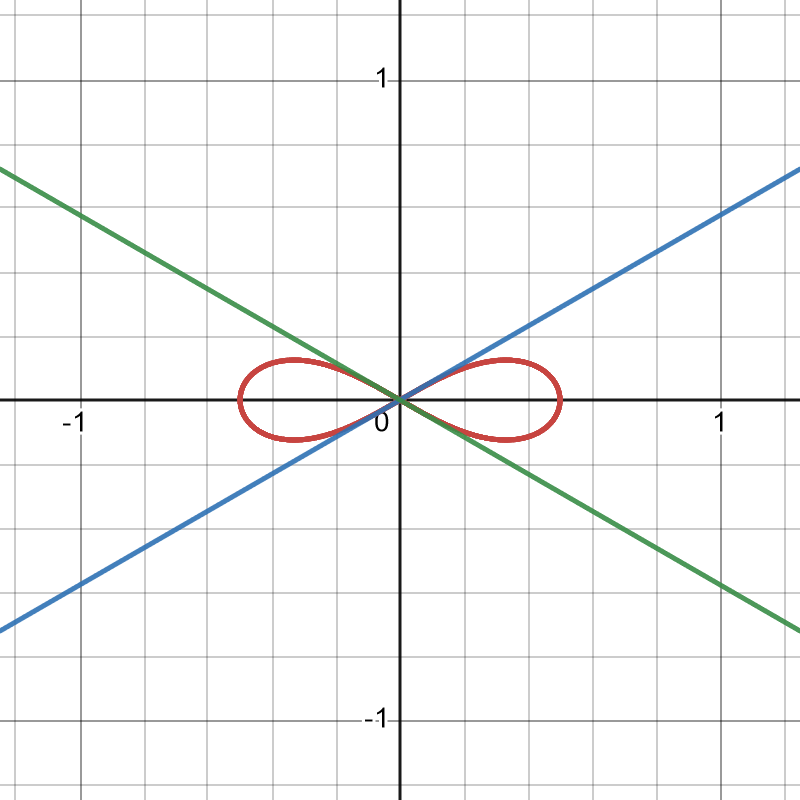
\includegraphics[scale=0.1]{desmos-graph(71).png}
           \end{center}
\end{solution}
\end{parts}


\end{questions}

\vfill 
\noindent \textbf{Optional} For extra fun, find a cartesian equation of the curve $\mathcal{C}$.
Show that for $x \in [-\frac{1}{2}, \frac{1}{2}]$, a cartesian
equation of the curve is $y = \pm \frac{\sqrt{\sqrt{64 {{x}^{2}}+9}-8 {{x}^{2}}-3}}{{{2}^{\frac{3}{2}}}}$.
And show that the other two solutions are not real. Finally,
are there any values of $x$ that allow the nested radical 
$\sqrt{\sqrt{64 {{x}^{2}}+9}-8 {{x}^{2}}-3}$ to denest?
    
\end{document}
